\begin{enumerate}[label=\thesubsection.\arabic*.,ref=\thesubsection.\theenumi]
\numberwithin{equation}{enumi}

\item
Consider a unity feedback system as shown in Fig.  \ref{fig:ee18btech11005}, with an integral compensator $\frac{k}{s}$ and open-loop transfer function
\begin{align}
G(s) = \frac{1}{s^2+3s+2}
\end{align}
where k greater than 0. 
%
Find its closed loop transfer function.
\begin{figure}[!ht]
	\begin{center}
		
		\resizebox{\columnwidth}{!}{A DC amplifier has an open loop gain of 1000 and two poles, a dominant one at 1kHz and a high frequency one whose location can be controlled. It is required to connect this amplifier in a negative feedback loop that provides a DC closed loop gain of 10 and a maximally flat response. 

\begin{enumerate}[label=\arabic*.,ref=\theenumi]
%\begin{enumerate}[label=\thesubsection.\arabic*.,ref=\thesubsection.\theenumi]
\numberwithin{equation}{enumi}
%\numberwithin{figure}{enumi}

\item Find the required value of $H$.
\\
\solution Table \ref{table:ee18btech11005_ Input_Table} summarises the given information.  The open loop gain can be expressed as
\begin{align}
\label{eq:ee18btech11005_open_loop_gain} 
  G(s) &= \frac{G_0}{\brak{1+\frac{s}{p_{1}}}\brak{1+\frac{s}{p_{2}}}} 
\\
\implies G(0) &= G_0
\end{align}
The closed loop gain 
\begin{align}
 \label{eq:ee18btech11005_transfer_function}
    T(s) &= \frac{G(s)}{1+G(s)H}
\\
\implies T(0) &= \frac{G_0}{1+G_0H}
\end{align}
%
Substituting from Table \ref{table:ee18btech11005_ Input_Table}, 
%But,also given DC closed loop gain is 10. DC closed loop gain is given in equation.\ref{eq:ee18btech11005_dc_gain} 
\begin{align}
\frac{1000}{1+1000H} &= 10
\\
\implies H &=  0.099 
\label{eq:ee18btech11005_h_value}
\end{align}
%
\begin{table}[!ht]
\centering
\input{./tables/ee18btech11005/ee18btech11005_1.tex}
\caption{1}
\label{table:ee18btech11005_ Input_Table}
\end{table}
\begin{align}
    G_0 &= 1000\\
\text{Therefore.,} G(s)&= \frac{1000}{(1+\frac{s}{p_{1}})(1+\frac{s}{p_{2}})}  
\end{align}
%Let, -p1 be the dominant pole.
%\begin{align}
%    p_1 &= 2\pi10^3 rad/sec
%\end{align}
%Now, we connect the system in a negative feedback of feedback factor H.
%------------------------------
\item Find $p_2$.
\\
\solution From \eqref{eq:ee18btech11005_transfer_function} and \eqref{eq:ee18btech11005_open_loop_gain},
\begin{align}
%    T(s) &= \frac{\frac{G_0}{(1+\frac{s}{p_{1}})(1+\frac{s}{p_{2}})}}{1+\frac{HG_0}{(1+\frac{s}{p_{1}})(1+\frac{s}{p_{2}})}}\\
%    T(s) &= \frac{\frac{p_1p_2G_0}{(p_1+s)(p_2+s)}}{1+\frac{p_1p_2HG_0}{(p_1+s)(p_2+s)}}
%\end{align}
%\begin{align}
%    T(s) &= \frac{p_1p_2G_0}{(p_1+s)(p_2+s) + p_1p_2HG_0}\\
%    T(s) &= \frac{p_1p_2G_0}{p_1p_2+(p_1+p_2)s+s^2 + p_1p_2HG_0}\\
    T(s) &= \frac{p_1p_2G_0}{s^2+(p_1+p_2)s+(HG_0+1)p_1p_2} \label{eq:ee18btech11005_closed_loop}
\\
&= \frac{K \omega_n^{2}}{s^2+2\zeta\omega_ns+\omega_n^{2}}
\\
%\label{eq:ee18btech11005_second_order_ce}
\implies 
\begin{split}
    \omega_n &= \sqrt{(HG_0+1)p_1p_2}\\
    \zeta &= \frac{p_1+p_2}{2\sqrt{(HG_0+1)p_1p_2}}
\end{split}
\label{eq:ee18btech11005_second_order_zeta}
\end{align}
using the standard forumulation for a second order system.  Also, for maximally flat response, the quality factor 
%Q of equation.\ref{eq:ee18btech11005_second_order_ce}, is given by
\begin{align}
    Q = \frac{1}{2\zeta}= \frac{1}{\sqrt{2}}&
\\
\implies  \zeta = \frac{1}{\sqrt{2}} &
\label{eq:ee18btech11005_second_order_zeta_q}
\\
\implies \frac{p_1+p_2}{2\sqrt{(HG_0+1)p_1p_2}} &= \frac{1}{\sqrt{2}}
%\end{align}
\\
%\begin{multline}
\implies \sqrt{\frac{p_1}{p_2}}+\sqrt{\frac{p_2}{p_1}} 
%\\
&= \sqrt{2(HG_0+1)} 
\end{align}
%\end{multline}
%
The above equation is of the form 
%
\begin{align}
\label{eq:ee18btech11005_x}
x + \frac{1}{x} &= a
\\
\implies x &= \frac{a \pm \sqrt{a^2 -4}}{2}
\label{eq:ee18btech11005_x_sol}
\end{align}
%
where 
\begin{align}
\label{eq:ee18btech11005_x_p1p2}
x  &= \sqrt{\frac{p_2}{p_1}}
\\
a &= \sqrt{2(HG_0+1)}, 
\label{eq:ee18btech11005_a}
\end{align}
Thus, from \eqref{eq:ee18btech11005_x_p1p2}, \eqref{eq:ee18btech11005_a}
and \eqref{eq:ee18btech11005_x_sol},
%
\begin{align}
p_2 &= p_1\sbrak{\frac{\sqrt{2\brak{HG_0+1}} \pm \sqrt{2 \brak{HG_0+1}-4}}{2}}^2
\end{align}
%
From the following code,
\begin{lstlisting}
codes/ee18btech11005/ee18btech11005_1.py
\end{lstlisting}
%
\begin{multline}
p_2 = 1244038.9567529503 
\\
\text{ and } 31.734068607786863
\end{multline}
%
%---------------------
\item  Draw the equivalent circuit system diagram.\\
\solution
The equivalent circuit system is shown in the figure.\ref{fig:equivalent_system}
\begin{figure}[!hbt]
	\begin{center}
			\resizebox{\columnwidth}{!}{\tikzstyle{block} = [draw, fill=blue!20, rectangle, 
    minimum height=3em, minimum width=6em]
\tikzstyle{sum} = [draw, fill=blue!20, circle, node distance=1cm]
\tikzstyle{input} = [coordinate]
\tikzstyle{output} = [coordinate]
\tikzstyle{pinstyle} = [pin edge={to-,thin,black}]

\begin{tikzpicture}[auto, node distance=2cm,>=latex']
    \node [input, name=input] {$V_s$};
    \node [sum, right of=input] (sum) {};
    \node [block, right of=sum] (controller) {$G$};
    \node [output, right of=controller] (output) {};
    \node [block, below of=controller] (feedback) {$H$};
    \draw [draw,->] (input) -- node {$V_s$} (sum);
    \draw [->] (sum) -- node {$V_i$} (controller);
    \draw [->] (controller) -- node [name=y] {$V_o$}(output);
    \draw [->] (y) |- (feedback);
    \draw [->] (feedback) -| node[pos=0.99]{$-$}  node [near end] {$V_f$} (sum);
\end{tikzpicture}
}
	\end{center}
\caption{1}
\label{fig:equivalent_system}
\end{figure}
%-----------------
\item Obtain $G(s)$ and $T(s)$
\\
\solution Substituting the value of $p_2$ in  \eqref{eq:ee18btech11005_open_loop_gain} and \eqref{eq:ee18btech11005_closed_loop},
\begin{align}
     G(s) &= \frac{1000}{(1+\frac{s}{2\pi10^3})(1+\frac{s}{1.244\times10^6})}
    \label{eq:ee18btech11005_G(s)}
\\
    T(s) &= \frac{10}{0.128\times10^{-11}s^2+1.599\times10^{-6}s+1}
    \label{eq:ee18btech11005_Transfer_func}
\end{align}
%-------------------
\item Verify from the Bode plot of above closed loop transfer function that it has maximally flat response.
\\
\solution The following code generates the bode plot of the transfer function in Fig. \ref{fig:ee18btech11005_1}.
\begin{lstlisting}
codes/ee18btech11005/ee18btech11005_2.py
\end{lstlisting}
\begin{figure}[!ht]
\centering
\includegraphics[width=\columnwidth]{./figs/ee18btech11005/ee18btech11005_1.eps}
\caption{}
\label{fig:ee18btech11005_1}
\end{figure}
%---------------------------------
\item Find the step response of $T(s)$
\\
\solution The following code generates the desired response of in Fig. \ref{fig:ee18btech11005_2}.
\begin{lstlisting}
codes/ee18btech11005/ee18btech11005_3.py
\end{lstlisting}
%
\begin{figure}[!ht]
\centering
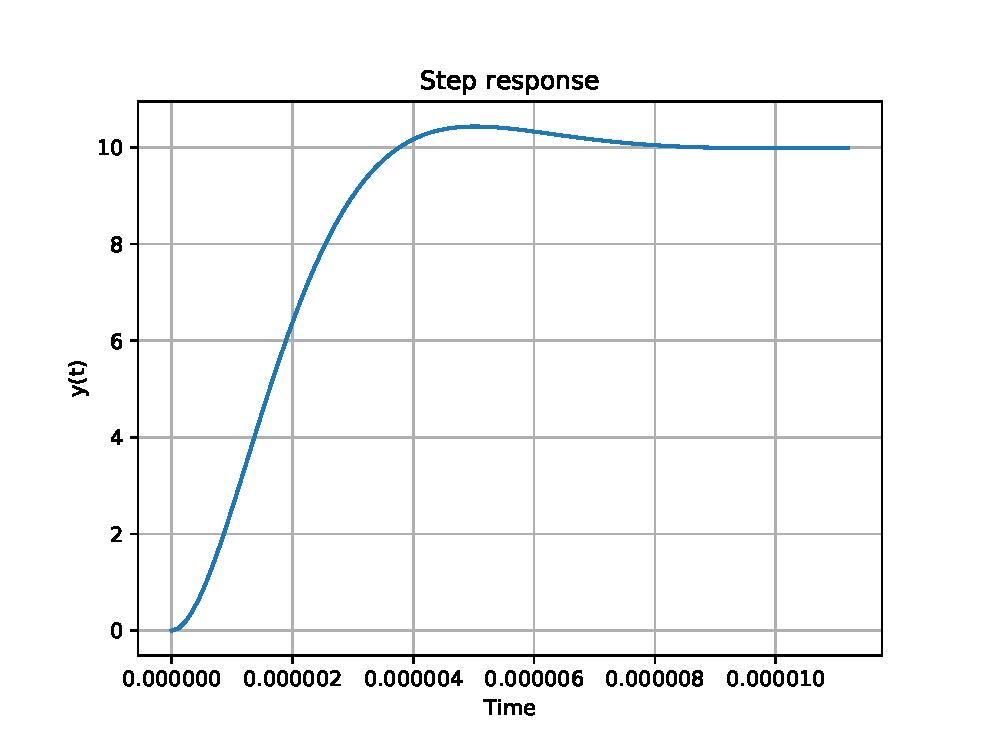
\includegraphics[width=\columnwidth]{./figs/ee18btech11005/ee18btech11005_2.eps}
\caption{}
\label{fig:ee18btech11005_2}
\end{figure}

%-------------------------------
\item Design a circuit that represents the above transfer function.\\
\solution The circuit can be designed using an operational amplifiers having negative feedback.Consider the circuit shown in figure.\ref{fig:equivalent_control_system}:1.Assume the gain of all the amplifiers are large.And assume no zero state response.Take the parameters in s-domain.\\
\begin{figure}[!hbt]
	\begin{center}
			\resizebox{\columnwidth}{!}{
 \begin{circuitikz}
\ctikzset{bipoles/length=1cm}

\draw 
(0, 0) node[op amp] (opamp) {}
(4.5, -0.35) node[op amp] (opamp2) {}
(9, -0.7) node[op amp] (opamp3) {}
(13,-1.05) node[op amp] (opamp4) {}
(opamp.-) -- (-1,0.35) -- (-1.5,0.35) to[R=$R_1$] (-3,0.35){}
(-1,0.35)-- (-1,1) to[R=$R_2$] (1.5,1) -- (1.5,0){}
(1.5,0)--(2,0) to[R=$R$] (3,0)--(3.5,0)--(opamp2.-){}
(opamp2.+)--(3.5,-0.7) node[ground]{}
(opamp.out)--(1.5,0){}
(opamp.+) -- (-1,-0.35) node[ground]{}
(3.5,0) -- (3.5,0.75)--(4,0.75) to[R=$R$] (6,0.75) -- (6,-0.35){}
(3.5,0.75)--(3.5,1.5) to[C=$C$] (6,1.5)--(6,0.35){}
(opamp2.out) -- (6,-0.35){}
(6,-0.35)--(6.5,-0.35) to[R=$R$] (7.5,-0.35)--(8,-0.35)--(opamp3.-){}
(opamp3.+)--(8,-1.05) node[ground]{}
(8,-0.35) -- (8,0.75) to[R=$R$] (10,0.75) -- (10,-0.7){}
(opamp3.out) -- (10,-0.7){}
(10,-0.7)--(10.5,-0.7) to[R=$R$] (11.5,-0.7)--(12,-0.7)--(opamp4.-) {}
(12,-0.7) -- (12,0.05) to[C=$C_1$] (14,0.05) -- (14,-1.05){}
(14,-1.05) -- (15,-1.05){}
(opamp4.out) -- (14,-1.05){}
(opamp4.+)--(12,-1.4) node[ground]{}
(3.5,0.75)--(3.5,2.5) to[R=$R$] (14,2.5) -- (14,-1.05){}
node at (-1,0.2){A}
node at (3.5,-0.2){B}
node at (8,-0.7) {C}
node at (12,-1){D}

node at (1.5,-0.4){$V_1$}
node at (6,-0.6){$V_2$}
node at (10,-1){$V_3$}
node at (15,-1.4) {$V_{out}$}
node at(-3,0.7){$V_{in}$}

;\end{circuitikz}



}
	\end{center}
\caption{1}
\label{fig:equivalent_control_system}
\end{figure}
\textbf{For the first amplifier..,}
Applying KCL at node A., 
Since, the opamp has large gain, potential at node A is assumed to be zero due to virtual short at node A.
\begin{align}
    \frac{0-V_{in}(s)}{R_1} +\frac{0-V_1(s)}{R_2} &= 0\\
    \frac{V_{in}(s)}{R_1} &= \frac{V_1(s)}{R_2}\\
\implies V_{in} &= -\frac{V_1(s) R_1}{R_2}\label{eq:ee18btech11005_opamp_1}
\end{align}
\textbf{For the second amplifier..,}
Applying KCL at node B..,
Similarly potential at node B is zero.
\begin{align}
  \frac{-V_1(s)}{R}+\frac{-V_2(s)}{R}-sCV_2(s)+\frac{-V_{out}(s)}{R} &= 0\\
  \frac{-V_1(s)}{R}+\frac{-V_2(s)}{R}-sCV_2(s) = \frac{V_{out}(s)}{R} \\
  \frac{-V_1(s)}{R} = V_2(s)\sbrak{sC+\frac{1}{R}}+\frac{V{out}(s)}{R} \label{eq:ee18btech11005_opamp_2}
\end{align}
\textbf{For the third amplifier..,}
Potential at node C is zero(Due to high gain of amplifier).Applying KCL at node C.
\begin{align}
    \frac{-V_2(s)}{R}+\frac{-V_3(s)}{R} = 0\\
    \implies V_2(s) = -V_3(s) \label{eq:ee18btech11005_opamp_3}
\end{align}
\textbf{For the Fourth amplifier.,}
Potential at node D is zero.Applying KCL at node D.
\begin{align}
    \frac{-V_3(s)}{R}+sC_1(-V_{out}(s)) = 0\\
    V_3(s) = -sC_1RV_{out}(s) \label{eq:ee18btech11005_opamp_4}
\end{align}
From equation.\ref{eq:ee18btech11005_opamp_4} and equation. \ref{eq:ee18btech11005_opamp_3}..,
\begin{align}
    V_2(s) = sC_1RV_{out}(s) \label{eq:ee18btech11005_eq_1}
\end{align}
Substituting the equation.\ref{eq:ee18btech11005_opamp_2} and equation.\ref{eq:ee18btech11005_eq_1},
\begin{align}
    \frac{-V_1(s)}{R} &= (s^2C_1CR + sC_1)V_{out}(s) +\frac{V_{out}(s)}{R}\\
    V_1(s) &= -(s^2C_1CR^2+sC_1R+1)V_{out}(s)\label{eq:ee18btech11005_eq_2}
\end{align}
from equation.\ref{eq:ee18btech11005_opamp_1} and equation.\ref{eq:ee18btech11005_eq_2}.
\begin{align}
     V_1(s) &= \frac{R_1}{R_2}(s^2C_1CR^2+sC_1R+1)V_{out}(s)\\
    \frac{V_{out}(s)}{V_{in}(s)} &= \frac{R_2}{R_1(s^2C_1CR^2+sC_1R+1)} \label{eq:ee18btech11005_eq_3}
\end{align}
Comparing equation.\ref{eq:ee18btech11005_Transfer_func} and equation.\ref{eq:ee18btech11005_eq_3}
\begin{align}
    \frac{R_2}{R_1} &= 10 \\
    C_1CR^2 &= 0.128x10^{-11} \\
    C_1R &= 1.599x10^{-6} F\\
\text{Let.,} R &= 1000 \Omega\\
\implies C_1 &= 1.599x10^{-9} \\
 \text{and.,} C_1CR^2 &= 0.128x10^{-11} \\
 \implies C &= 0.8005x10^{-9} F
\end{align}
\begin{align}
\text{Let..,} R_1 &= 100\Omega\\
\implies R_2 &= 1000\Omega
\end{align}
\begin{table}[!ht]
\centering
\input{./tables/ee18btech11005/ee18btech11005_2.tex}
\caption{1}
\label{table:ee18btech11005_ Output_Table}
\end{table}
From Table.\ref{table:ee18btech11005_ Output_Table}:1. The Final circuit is shown in figure.\ref{fig:Final_circuit}
\begin{figure}[!hbt]
	\begin{center}
			\resizebox{\columnwidth}{!}{\begin{circuitikz}
\ctikzset{bipoles/length=1cm}

\draw 
(0, 0) node[op amp] (opamp) {$1$}
(4.5, -0.35) node[op amp] (opamp2) {$2$}
(opamp.-) -- (-1,0.35) -- (-1.5,0.35) to[R=$1k\Omega$] (-3,0.35){}
(-1,0.35)-- (-1,1) to[C=$1nF$] (1.5,1) -- (1.5,0){}
(1.5,0)--(2,0) to[R=$1k\Omega$] (3,0)--(3.5,0)--(opamp2.-){}
(opamp2.+)--(3.5,-0.7) node[ground]{}
(opamp.out)--(1.5,0){}
(opamp.+) -- (-1.5,-0.35) -- (-1.5,-1.5) 
(6,-1.5) to[C=$0.599nF$] (6,-3) node[ground]{}
(-1.5,-1.5) to[R=$1k\Omega$] (6,-1.5) --(6,-0.35){}
(3.5,0) -- (3.5,0.75)--(4,0.75) to[C=$0.681nF$] (6,0.75) -- (6,-0.35){}
(opamp2.out) -- (6,-0.35){}
(6,-0.35)--(6.5,-0.35)
node at (-1,0.2){A}
node at (3.5,-0.2){B}
node at (1.5,-0.4){$V_1$}
node at (6.3,-0.6){$V_{out}$}
node at(-3,0.7){$V_{in}$}

;\end{circuitikz}

}
	\end{center}
\caption{1}
\label{fig:Final_circuit}
\end{figure}
%--------------------------------------------
\item Draw the equivalent block diagram of the above circuit.\\
\solution The equivalent block diagram is shown in the Fig.\ref{fig:ee18btech11005_4}.The block diagram can be computed similarly from the above circuit diagram. Where each opamp is reduced into a block. And the last three blocks having a negative feedback.
\begin{figure}[!ht]
	\begin{center}
			\resizebox{\columnwidth}{!}{\tikzstyle{block} = [draw, fill=blue!20, rectangle, 
    minimum height=3em, minimum width=4em]
\tikzstyle{sum} = [draw, fill=blue!20, circle, node distance=1cm]
\tikzstyle{input} = [coordinate]
\tikzstyle{output} = [coordinate]
\tikzstyle{out} = [coordinate]
\tikzstyle{pinstyle} = [pin edge={to-,thin,black}]
\begin{tikzpicture}[auto, node distance=2cm]
    \node [input, name=input] {};
    \node [block, right of=input] (control) {$\frac{-R_2}{R_1}$};
    \node [right of=control](out) {};
    \node [sum, right of=out] (sum) {};
    \node [block, right of=sum] (controller1) {$\frac{-R}{R(sRC+1)}$};
    \node [block, right of=controller1] (controller2) {$-1$};
    \node [block, right of=controller2] (controller3) {$\frac{-1}{sC_1R}$};
    \node [output, right of=controller3] (output) {};
    \node [block, below of=controller2] (feedback) {$\frac{1}{2}$};
    \draw [draw,->] (input) -- node {$V_s$} (control);
    \draw [->] (control) -- node {}(sum);
    \draw [->] (sum) -- node {$V_i$} (controller1);
    \draw [->] (controller1) -- node {} (controller2);
    \draw [->] (controller2) -- node {} (controller3);
    \draw [->] (controller3) -- node [name=y] {$V_o$}(output);
    \draw [->] (y) |- (feedback);
    \draw [->] (feedback) -| node[pos=0.99]{$-$}  node [near end] {$V_f$} (sum);
\end{tikzpicture}
}
	\end{center}
\caption{}
\label{fig:ee18btech11005_4}
\end{figure}
%------------------------------------------------
\item Verify the closed loop DC gain using NGSPICE simulator.
\\
\solution 
The following README file gives the procedure to be followed.
\begin{lstlisting}
codes/ee18btech11005/spice/README
\end{lstlisting}
From equation.\ref{eq:ee18btech11005_Transfer_func}.
The DC closed loop gain is 10.\\
The following netlist file, gives the DC gain of the closed loop function.
\begin{lstlisting}
codes/ee18btech11005/spice/gvv_ngspice.net
\end{lstlisting}
We can observe from simulation that the value of DC closed loop gain is 9.997.\\
\textbf{Error analysis:-}\\
ERROR in DC GAIN = 10-9.993 = 0.007
Thus, the predicted value in ngspice is almost accurate.
Therefore, the value is verified using ngspice.
%--------------------------------
\item Verify the step response of the output from ngspice simulation.\\
\solution The following netlist file does the transient anaylsis and store the Vout values with respect to time in a dat file. 
\begin{lstlisting}
codes/ee18btech11005/spice/gvv_ngspice2.net
\end{lstlisting}
Following python code is to plot the step response.
\begin{lstlisting}
codes/ee18btech11005/spice/ee18btech11005_spice.py
\end{lstlisting}
The step response obtained is shown in the figure.\ref{fig:ee18btech11005_3}.The graph has steady state value equal to 10.
\begin{figure}[!ht]
\centering
\includegraphics[width=\columnwidth]{./figs/ee18btech11005/ee18btech11005_spice.eps}
\caption{}
\label{fig:ee18btech11005_3}
\end{figure}

\end{enumerate}
}
	\end{center}
\caption{}
\label{fig:ee18btech11005}
\end{figure}

\solution $\because H(s) = 1$ in Fig.  \ref{fig:ee18btech11005}, due to unity feedback,   the transfer function is given by
\begin{align}
\frac{Y(s)}{X(s)} &= \frac{G(s)}{1+G(s)H(s)}
\\
\implies T(s) &= \frac{k}{s^3+3s^2+2s}
\end{align}
%
\item Find the {\em characteristic} equation for $G(s)$.
\\
\solution The characteristic equation is
\begin{align}
\label{eq:routh_char_eq}
 1 + G(s)H(s) &= 0 
\\
\implies 1 + \sbrak{\frac{k}{s^3+3s^2+2s}} &= 0
\\
\text{or, } s^3+3s^2+2s+k &= 0
\end{align}
\item Using the tabular method for the Routh hurwitz criterion, find $k > 0$ for which there are two poles of unity feedback system on j${\omega}$ axis.
%
\\
\solution 
This criterion is based on arranging the coefficients of characteristic equation into an array called Routh array.
For any characteristic equation 
\begin{multline}
q(s) = a_0s^n+a_1s^{n-1}+.....+a_{n-1}s+a_n = 0
\end{multline}
the Routh array can be constructed as 
 
\begin{align}
\mydet{s^n\\s^{n-1}\\s^{n-2} \\ \vdots}
 \mydet{a_0 & a_2 & a_4 & \cdots \\
a_1 & a_3 & a_5 & \cdots  \\
b_1 & b_2 & b_3 & \cdots \\
\vdots & \vdots & \vdots & \ddots &\vdots 
 \cdots \\}
\end{align}
%
 where
 \begin{align}
 b_1 =\frac{ a_1a_2-a_0a_3}{a_1}  
 \\
 b_2 =\frac{ a_1a_4-a_0a_5}{a_1} 
 \\
 c_1=\frac{ b_1a_3-a_1b_2}{b_1} 
\\
 c_2=\frac{ b_1a_5-a_1b_3}{b_1}  
\end{align}
For poles to lie on imaginary axis any one entire row of hurwitz matrix should be zero.
Constructing the routh array for the characteristic equation obtained in \ref{eq:routh_char_eq},
%
\begin{align}
 s^3+3s^2+2s+k = 0
\end{align}
%
\begin{align}
\mydet{s^3\\s^2\\s^1 \\ s^0}
\mydet{1 & 2 \\ 3 & k \\  \frac{6-k}{3} & 0\\ k & 0}
\end{align}
For poles on $\j \omega$ axis any one of the row should be zero.
%
\begin{align}
\therefore \frac{6-k}{3} &= 0 \text{ or } k = 0
\\
\implies k &= 6 \quad \because k > 0
\end{align}
\item Repeat the above using the determinant method.
\\
\solution The {\em Routh matrix} can be expressed as
\begin{align}
\vec{R} = \myvec{a_0 & a_2 & a_4 & \cdots \\
a_1 & a_3 & a_5 & \cdots  \\
 0 & a_0 & a_2\cdots \\
 0 & a_1 & a_3 \cdots\\
\vdots & \vdots & \vdots & \ddots &\vdots 
\cdots \\}
\end{align}
and the corresponding Routh determinants are
\begin{align}
D_1 &= |a_0|
\\
D_2 &= 
\mydet{
a_0 & a_2 
\\ 
a_1 & a_3
} 
\\
D_3 &=\mydet{
a_0 & a_2 & a_4 
\\ a_1 & a_3 & a_5 
\\ 0 & a_0 & a_2}
\\
\dots
\end{align}
If at least any one of the Determinents are zero then the poles lie on imaginary axes.  From \eqref{eq:routh_char_eq},
%
\begin{align}
D_1 &= 1 \ne 0
\\
D2 &= \mydet{
1 & 2 \\ 3 & k } 
&= k-6 =0 \implies k = 6
\end{align}
%
\item Verify your answer using a python code for both the determinant method as well as the tabular method.
\label{prob:ee18btech11005_python}
\\
\solution 
The following code verifies the stability using the tabular method 
%
\begin{lstlisting}
codes/ee18btech11005_2.py
\end{lstlisting}
and the following one verifies using the determinant method.
\begin{lstlisting}
codes/ee18btech11005.py
\end{lstlisting}
%
provides the necessary soution.
\begin{itemize}
\item  For the system to be stable all coefficients should lie on left half of s-plane. Because if any pole is in right half of s-plane then there will be a component in output that increases without bound,causing system to be unstable.
All the coefficients in the characteristic equation should be positive.This is necessary condition but not sufficient.Because it may have poles on right half of s plane.
Poles are the roots of the characteristic equation.
    \item A system is stable if all of its characteristic modes go to finite value as t goes to infinity.It is possible only if all the poles are on the left half of s plane.
    The characteristic equation should have negative roots only. So the first column should always be greater than zero.That means no sign changes.
    \item A system is unstable if its characteristic modes are not bounded. Then the characteristic equation will also have roots in the right side of s-plane.That means it has sign changes.
    \end{itemize}

\end{enumerate}\begin{enumerate}[label=\thesection.\arabic*.,ref=\thesection.\theenumi]
\numberwithin{equation}{enumi}

\item
Consider a unity feedback system as shown in the figure,shown with an integral compensator k/s and open-loop transfer function
\begin{align}
G(s) = \frac{1}{s^2+3s+2}
\end{align}
where k greater than 0. The positive value of k for which there are two poles of unity feedback system on j${\omega}$ axis is equal to-----(rounded off to two decimal places)
%\centering
%\includegraphics[width=\columnwidth]{ee18btech11005.eps}
\begin{figure}
\centering
\includegraphics[width=\columnwidth]{figure.eps}
\end{figure}
\solution The transfer function for negative feedback is given by
\begin{align}
\frac{Y(s)}{X(s)} &= \frac{G(s)}{1+G(s)H(s)}
\end{align}
where H(s) = 1 for unity feedback system
and G(s) is net forward open loop gain
\begin{align}
G(s) &=  \sbrak{\frac{1}{s^2+3s+2}}\sbrak{\frac{k}{s}}
&= \frac{k}{s^3+3s^2+2s}
\end{align}
Characteristic equation is..,
\begin{align}
 1 + G(s)H(s) = 0 \label{eq:sec_order_op}
\\
=> 1 + \sbrak{\frac{k}{s^3+3s^2+2s}} = 0
\\
=> s^3+3s^2+2s+k = 0
\end{align}
The Routh hurwitz criterion:-
This criterion is based on arranging the coefficients of characteristic equation into an array called Routh array.
For any characteristic equation q(s),
\begin{multline}
q(s) = a_0s^n+a_1s^{n-1}+.....+a_{n-1}s+a_n = 0
\end{multline}
Routh array can be constructed as follows..,
 
\myvec{s^n\\s^{n-1}\\s^{n-2} \\ \vdots}
 \myvec{a_0 & a_2 & a_4 & \cdots \\
a_1 & a_3 & a_5 & \cdots  \\
b_1 & b_2 & b_3 & \cdots \\
\vdots & \vdots & \vdots & \ddots &\vdots 
 \cdots \\}
 \\
 where
 \begin{align}
 b_1 =\frac{ a_1a_2-a_0a_3}{a_1}  
 \\
 b_2 =\frac{ a_1a_4-a_0a_5}{a_1} 
 \\
 c_1=\frac{ b_1a_3-a_1b_2}{b_1} 
\\
 c_2=\frac{ b_1a_5-a_1b_3}{b_1}  
\end{align}
For poles to lie on imaginary axis any one entire row of hurwitz matrix should be zero.
Constructing the routh array for the characteristic equation obtained in equation(\ref{eq:sec_order_op})
\begin{align}
 s^3+3s^2+2s+k = 0
\end{align}
%
\begin{align}
\myvec{s^3\\s^2\\s^1 \\ s^0}
\myvec{1 & 2 \\ 3 & k \\  \frac{6-k}{3} & 0\\ k & 0} \label{eq:sec_order_op_1}
\end{align}
For poles on j$\omega$ axis any one of the row should be zero.
\begin{align}
\frac{6-k}{3} = 0 \hspace{5pt} or\hspace{5pt} k = 0
\end{align}
But given k greater than 0 ...
\begin{align}
   6-k = 0\\
   k = 6
\end{align}
\item Repeat the above using the determinant method.
\solution
Determinent method:
\myvec{a_0 & a_2 & a_4 & \cdots \\
a_1 & a_3 & a_5 & \cdots  \\
 0 & a_0 & a_2\cdots \\
 0 & a_1 & a_3 \cdots\\
\vdots & \vdots & \vdots & \ddots &\vdots 
\cdots \\}
\begin{align}
D1 &= |a_0|
\\
D2 &= \begin{vmatrix}
a_0 & a_2 \\ a_1 & a_3 \end{vmatrix}
\\
D3 &=\begin{vmatrix}
a_0 & a_2 & a_4 \\ a_1 & a_3 & a_5 \\ 0 & a_0 & a_2 \end{vmatrix}
\end{align}
and so on...
If atleast any one of the Determinents are zero then the poles lie on imaginary axes.
So,For the given question the routh array is obtained from equation(\ref{eq:sec_order_op})
\begin{align}
D1 &= 1
\\
D2 &= \begin{vmatrix}
1 & 2 \\ 3 & k \end{vmatrix} 
&= k-6
\\
D3 &=\begin{vmatrix}
1 & 2 & 0 \\ 3 & k & 0 \\ 0 & 1 & 2 \end{vmatrix}
&=2k-12
\end{align}
D2 = k-6 =0 for the poles to lie on imaginary axis
\begin{align}
   k-6 = 0\\
   k = 6
\end{align}
\item Verify your answer using a python code for both the determinant method as well as the tabular method.
\solution 
The following code 
%
\begin{lstlisting}
codes/ee18btech11005/routhhurwitztabular.py
\end{lstlisting}
\item Why the sign change in routh array determine stability?
\solution For the system to be stable all coefficients should lie on left half of s-plane. Because if any pole is in right half of s-plane then there will be a component in output that increases without bound,causing system to be unstable.
All the coefficients in the characteristic equation should be positive.This is necessary condition but not sufficient.Because it may have poles on right half of s plane.
Poles are the roots of the characteristic equation.
\begin{itemize}
    \item A system is stable if all of its characteristic modes go to finite value as t goes to infinity.It is possible only if all the poles are on the left half of s plane.
    The characteristic equation should have negative roots only. So the first column should always be greater than zero.That means no sign changes.
    \item A system is unstable if its characteristic modes are not bounded. Then the characteristic equation will also have roots in the right side of s-plane.That means it has sign changes.
    \end{itemize}
\end{enumerate}
